\documentclass[a4paper, 12pt]{article}

% Package digunakan dalam dokumen laporan dan constraint
\usepackage[a4paper, margin=1in]{geometry}
\usepackage{tabularx}
\usepackage[utf8]{inputenc}
\usepackage{graphicx}
\usepackage{booktabs}
\usepackage{array}
\usepackage[bahasa]{babel}
\usepackage{setspace}
\onehalfspacing
\usepackage{float}
\usepackage{enumitem}

%awal 
\begin{document}

%Halman Judul 
\begin{titlepage}
    \centering
    \vspace*{\stretch{1.0}}
    
    {\Huge\bfseries Laporan Ujian Tengah Semester\par}
    \vspace{0.5cm}
    {\LARGE\bfseries Keamanan, Kesehatan, Keselamatan, dan Lingkungan Kerja Industri (K3L)\par}
    
    \vspace{2.5cm}
    %logo itera 
    \begin{figure}[htbp] 
        \centering
        
\includegraphics[width=0.4\linewidth]{Logo_ITERA.png}
        \label{fig:logo}
    \end{figure}
    {\large Disusun oleh:\par}
    \vspace{0.5cm}
    {\Large Nama Mahasiswa: Muhammad Daffa Hakim Matondang\par}
    {\Large NIM: 123140002\par}
    
    \vspace{\stretch{2.0}}    
    {\large\bfseries Program Studi Teknik Informatika\par}
    {\large\bfseries Institut Teknologi Sumatera\par}
    \vspace{0.5cm}
    {\large Dosen Penguji:\par}
    {\large Amrina Mustaqim, S.Si., M.T.\par}
    {\large Hesti Wahyu Handani, S.Si., M.Si.\par}
    \vspace{0.5cm}
    {\large \today\par} 
    \vspace*{\stretch{1.0}}
\end{titlepage}



%Bab 1 
\section{Konsep dan Peran K3L}
\noindent\textbf{Judul Kasus:} Analisis Risiko dan Mitigasi Bahaya Fisik Akibat Jalan Trotoar Berlubang di Area Pejalan Kaki Depan Asrama TB5

\subsection{Deskripsi Situasi}
Untuk deskripsi situasi sendiri itu bisa dilihat bahwasannya kondisi didepan asrama TB 5 sendiri itu di trotoar untuk pejalan kaki terjadi kerusakan parah yang berupa lubang besar akibat tanah yang ada dibawah amblas dan terjadilah longsor kecil. dari kondisi tersebut dapat berpotensi menimbulkan adanya kecelakaan bagi pejalan kaki di sekitar asrama TB 5 , apalagi waktu di malam hari ataupun pada saat kondisi di daerah tersebut hujan. Area disekitar situ pun tidak ada peringatan atau pembatas pengaman.
\subsection{Analisis Konsep K3L}
Nah seperti yang kita ketahui K3L ini sendiri terbentuk dari 3 aspek utama kan yaitu ada keselamatan kerja , kesehatan kerja kemudian yang terakhir itu ada perlindungan lingkunnya seperti apa mungkin untuk penjelasan secara lanjut bisa saya jelaskan dibawah ini:
\begin{itemize}
    \item \textbf{Keselamatan Kerja (Safety):} Poin ini mengharuskan kita untuk berpikir lebih mendalam tentang masalah yang ada yaitu kerugian fisik yang disebabkan oleh trotoar yang runtuh dan tergelincir, seperti yang disebutkan dalam deskripsi situasi. Dari risiko yang diuraikan, seseorang dapat dengan mudah menyimpulkan bahwa lubang besar di trotoar bisa menyebabkan cedera yang sangat merugikan bagi pejalan kaki di dekat asrama TB 5, karena kedalaman lubang tersebut. Dalam hal ini, cedera semacam itu bisa dengan mudah merupakan hasil dari tidak adanya langkah-langkah keselamatan. Dimungkinkan untuk membangun dan menerapkan langkah-langkah keselamatan dalam hal ini melalui penempatan tanda peringatan sederhana, yang selanjutnya dapat memungkinkan penyelesaian pekerjaan yang diperlukan untuk menutup lubang-lubang tersebut.


    \item \textbf{Kesehatan Kerja (Health):} Pada poin ini ya kita bisa lihat sudah jelas di area tersebut itu sangat berbahaya karena lubang yang ada cukup dalam otomatis siapapun yang jatuh akibat lubang tersebut bisa mengalami cedera di bagian otot , dan luka robek yang cukup parah. Hal ini juga membuat para pejalan kaki menjadi ada timbul rasa tidak aman ketika lewat di daerah tersebut.Untuk cara pencegahan mungkin bisa dengan langkah kecil yaitu menjaga kebersihan di daerah tersebut dan juga membuat jalur alternatif sembari jalan trotoar diperbaiki.
    \item \textbf{Perlindungan Lingkungan:} Nah sekarang pada poin ini kita lihat kembali akibat dari permasalahan yang ada yaitu lubang dalam akibat longsor itu sudah sangat menunjukkan adanya gangguan struktur drainase yang kurang bagus dan struktur tanah yang tidak stabil.Perlindungan yang bisa dilakukan ya sudah jelas harus diperbaiki sistem drainase nya bagaimana , kemudian di tinjau ulang penataan struktur tanahnya seperti apa , agar lingkungan tetap stabil dan aman.
\end{itemize}

\subsection{Peran K3L di Industri}
Pada poin ini K3L berperan cukup penting dalam menjamin keselamatan semua masyrakat kampus seperti mahasiswa , dosen , dan tenaga pendidikan agar berlangsung aman , sehat dan juga nyaman. Karena disini konteks industri ini merujuk ke kampus ITERA itu sendiri maka adapun dengan diadakannya K3L ini mencegah terjadinya:
\begin{enumerate}
    \item \textbf{Kecelakaan:} Contohnya ya seperti yang sudah di mention pada bagian sebellumnya yaitu jatuh akibat trotoar nya berlubang.
    \item \textbf{Cara Pencegahan:} Untuk cara pencegahan sendiri bisa melalui inspeksi rutin , perbaikan Infrastruktur dan mungkin yang paling membantu disini yaitu dengan adanya pemasangan rambu tanda bahaya disekitar area lubang. 
\end{enumerate}
Sesuai penjelasan sebelumnya, kami juga mempercayakan kepada K3L untuk menjaga agar lingkungan Kampus ITERA tetap rapi, teratur, dan tidak rusak, sehingga aman bagi orang-orang yang berada di sekitar kampus.


\subsection{Strategi Komunikasi}
Dalam hal ini, strategi komunikasi dapat melibatkan memberi tahu pihak yang bertanggung jawab untuk K3L di ITERA tentang kondisi berbahaya sehingga mereka dapat memasang penghalang dan tanda peringatan di sekitar lokasi dengan lubang di depan asrama TB 5. Untuk tujuan komunikasi, informasi juga dapat dibagikan melalui saluran media sosial kampus, seperti Instagram, sehingga komunitas kampus mendapat pembaruan. Terakhir, saya berharap bahwa kondisi berbahaya di sekitar lubang akan diperbaiki tepat waktu.


%Bab 2 
\section{Regulasi dan Standar K3L}
\noindent\textbf{Judul Kasus:}  Analisis Risiko dan Mitigasi Bahaya Fisik Akibat Jalan Trotoar Berlu-
bang di Area Pejalan Kaki Depan Asrama TB5

\subsection{Analisis Keterkaitan Regulasi}
Kondisi bahaya pada kasus ini relevan dengan beberapa regulasi dan standar K3L, antara lain:
\begin{itemize}
    \item \textbf{Standar Nasional Indonesia (SNI) 8153:2015:} Nah jika kita berkaca pada regulasi ini dan melihat isinya yaitu untuk menetapkan spesifikasi teknis desain trotoar , termasuk ketahanan terhadap beban dan keaadaan permukaan jalan maka ini nyambung dengan case masalah yang sya bawakan yaitu jalan trotoar yang berlubang jadi tidak sesuai dengan regulasi SNI ini.
    \item \textbf{ISO 21542:2021 Building Construction Accesibility and usability of the built environment:} Pada regulasi atau peraturan ini standar biasanya mengatur untuk aksesibilitas bangunan dan lingkungan binaan agar bisa digunakan orang. Nah jika kita coba trackback ke masalah yang saya bawa trotoar yang berlubang ini sudah pastilah mengurangi aksesibilitas dan keamanan pejalan kaki di sekitar lingkungan kampus ITERA terutama didepan asrama TB 5.
\end{itemize}

\subsection{Langkah Perbaikan Sistem}
Perbaikan secara sistematis dapat dilakukan menggunakan \textit{Plan-Do-Check-Act} (PDCA):
\begin{description}
    \item[Plan] Untuk rencana mungkin bisa dengan pencobaan untuk melakukan perbaikan Lubang yang sangat dalam itu dengan cara pengadaan proyek perbaikan.
    \item[Do] untuk poin DO ini ya pelaksanaan dari proyek itu sendiri secara teknisnya mungkin seperti perbaikan struktur trotoar, memperbaiki drainase nya seperti apa , serta pemasangan rambu bahaya atau garis pembatas agar orang-orang kampus ITERA tahu ada bahaya.
    \item[Check] Pada poin check ini akan dilakukannya peninjauan kembali untuk memvalidasi dan pengecekan ulang apakah area tersebut sudah aman untuk dilewati oleh pejalan kaki.
    \item[Act] Pada bagian ini kurang lebih seperti maintenance proyek dalam berkelanjutan pemeliharaannya seperti apa nantinya dan juga bisa mensosisalisasikan K3L kepada Masyarakat Kampus ITERA. 
\end{description}

\subsection{Peran Komunikasi \& Pelatihan}
Untuk komunikasi sendiri ya sudah pasti sangat berperan penting disini untuk penyebaran informasi bahaya akibat dari lubang yang dalam tersebut.dan juga penting agar pihak yang berwenang dalam K3L di ITERA bisa cepat mengatasi masalah tersebut.Dan juga untuk pelatihan bisa diberikan kepada Mahasiswa , Dosen , dan Tendik ITERA agar memahami dan kenal terhdap bahaya fisik itu seperti apa , cara pelaporan kondisi yang tidak aman seperti apa.
%Bab 3 
\section{Identifikasi Bahaya dan Analisis Risiko}

\subsection{Identifikasi Jenis Bahaya}
Jenis bahaya dari bahaya ini adalah adalah \textbf{Bahaya Fisik}. Bahaya ini berasal dari Lubang yang danagat dalam akibat dari longsor dan amblas didepan asrama TB 5 ITERA.
\subsection{Analisis Risiko}

\begin{table}[H]
    \centering
    \caption{Tabel Analisis Risiko pada Lubang didepan Asrama TB 5}
    \label{tab:risiko}
    \fontsize{8pt}{10pt}\selectfont
    \begin{tabularx}{\textwidth}{>{\centering\arraybackslash}p{0.7cm} 
                                   >{\centering\arraybackslash}p{1.3cm} 
                                   >{\raggedright\arraybackslash}p{2.5cm} 
                                   >{\raggedright\arraybackslash}p{2.2cm} 
                                   >{\centering\arraybackslash}p{1.1cm} 
                                   >{\centering\arraybackslash}p{1.1cm} 
                                   >{\centering\arraybackslash}p{1.2cm} 
                                   >{\raggedright\arraybackslash}X}
        \toprule
        \textbf{No} & \textbf{Jenis Bahaya} & \textbf{Sumber Bahaya} & \textbf{Potensi Akibat} & \textbf{Nilai\ Kemung\-kinan} & \textbf{Nilai\ Kepa\-rahan} & \textbf{Tingkat Risiko} & \textbf{Rekomendasi Pengendalian} \\
        \midrule
        1 & Fisik & Bahaya fisik akibat dari lubang dalam pada trotoar didepan asrama TB 5 & 
        Cedera Berat seperti patah tulang dan luka sobek pada fisik.
        & 4 & 4 & 16 (Tinggi) & 
        \textbf{1.} Rekayasa Teknik: Pemasangan garis pembatas bahaya sementara, rambu bahaya juga diperlukan disini. 
        \newline
        \textbf{2.} Administratif: Pengadaan sosialaisasi pentingnya aware kepada hal yang membhaayakan seperti case lubang dalam yang disebabkan struktur tanah longsor dan ambruk dan segera laukakn pengaduan ke pihak K3L ITERA. \\
        \bottomrule
    \end{tabularx}
\end{table}

\subsection{Alat Bantu Identifikasi Bahaya}
Metode atau alat bantu yang digunakan untuk mengidentifikasi bahaya ini adalah :
\begin{enumerate}
    \item \textbf{Checklist Inspeksi K3L:} Melakukan pengecekan berkala dan berulang untuk pemeliharaan di sekitar lingkungan kampus ITERA.dan juga melakukan dokumentasi foto biar terdata konkrit dan jelas.
    \item \textbf{Laporan Bahaya (\textit{Hazard Reporting}):} Gunanya sebagai pelaporan temuan bahaya.
\end{enumerate}


%Bab 4 
\section{Penerapan SOP \& Sikap Akademik}

\subsection{Rancangan Singkat SOP untuk kasus yang telah anda pilih}

\begin{table}[H]
    \centering
    \caption{SOP: Penanganan Bahaya Fisik pada Area Trotoar Asrama TB 5 ITERA}
    \label{tab:sop}
    \begin{tabularx}{\textwidth}{>{\centering\arraybackslash}p{1.5cm} 
                                  >{\raggedright\arraybackslash}X 
                                  >{\centering\arraybackslash}p{3cm} 
                                  >{\centering\arraybackslash}p{3cm}}
        \toprule
        \textbf{Langkah} & \textbf{Deskripsi Tindakan} & \textbf{Penanggung Jawab} & \textbf{Alat yang Digunakan} \\
        \midrule
        1 & Identifikasi lokasi trotoar berlubang dan di dokumentasiin seperti apa kondisi bahaya nya. & Tim K3L ITERA & Kamera , Form Inspeksi \\
        \addlinespace
        2 & Memasang rambu peringatan dan pemabtas di area berbahaya agar mencgah pejalan kaki melewati area tersebut & Tim K3L  & cone , papan peringatan \\
        \addlinespace
        3 & Melakukan Koordinasi dengan bagian sarana prasarana untuk perbaikan permanen trotoar dan drainase. & Tim K3L dan sarpras & Alat Konstruksi, material perbaikan \\
        \addlinespace
        4 & Melakukan inspeksi ulang pasca perbaikan untuk memastikan area aman digunakan & Tim K3L & Form Evaluasi, Kamera \\
        \bottomrule
    \end{tabularx}
\end{table}

\subsection{Sikap Akademik dan Komunikatif}
Pada bagian ini Mahasiswa dan masyarakat kampus ITERA yang lainnya harus bisa menerapkan sikap peduli, tanggap dan bertanggung jawab terhadap keselamatan di area kampus kita sendiri, ITERA tercinta.Dalam case trotoar berlubang ini sudah sangat jelas ini sangat mengganggu pejalan kaki sedangkan pengguna trotoar itu sendiri tidak lain dan tidak bukan ya mahasiswa dan dosen dan juga Tendik. Maka dari itu harus aware dan peduli dengan melakukan pelaporan kepada pihak K3L ITERA.Dan juga perlu sikap komunikatif dengan pengkoordinasian yang sopan, jelas dan tepat antara masyarakat kampus seperti mahasiswa , dosen , dan tendik. Supaya masalah cepat teratasi
\end{itemize}
\section{Lampiran}
\begin{enumerate}
  \item Gambar Kondisi 

  \begin{figure}[H]
    \centering
    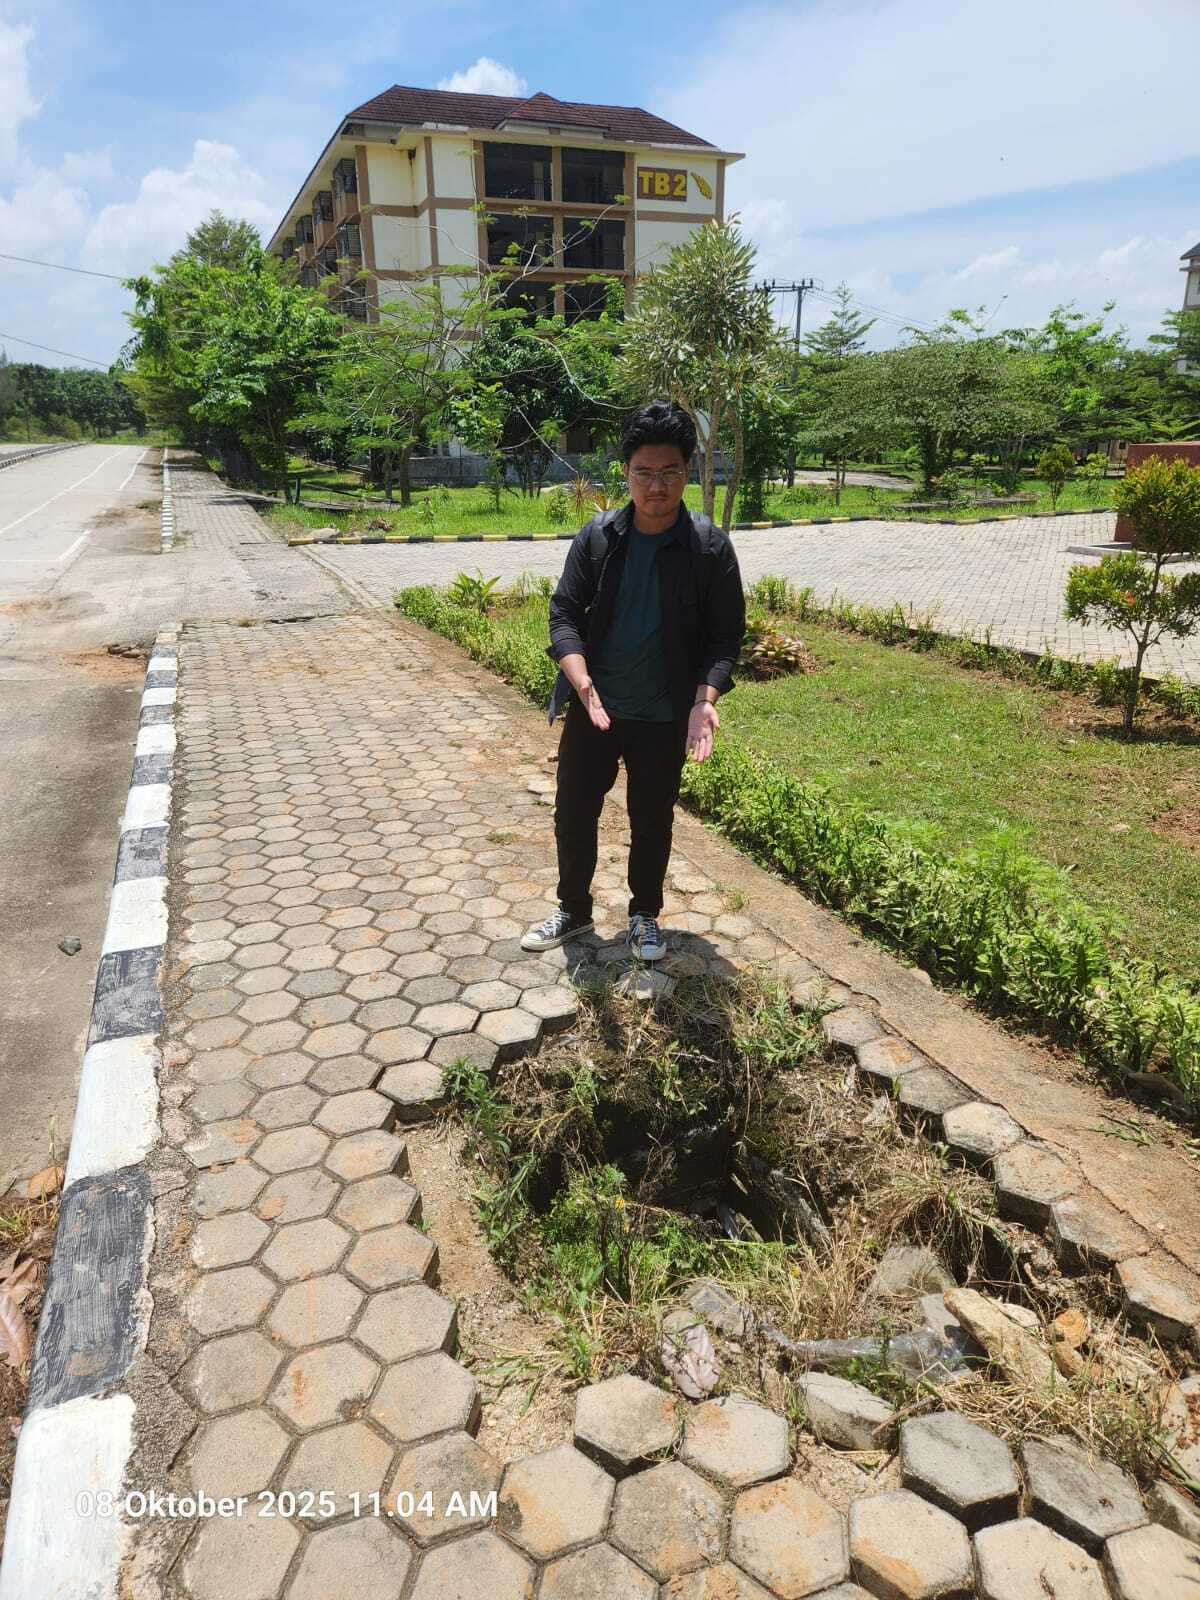
\includegraphics[width = .5\linewidth]{kondisi_lapangan_new.png}
    \caption{Kondisi Lapangan}
  \end{figure}  
\item Link repository GitHub : 
\url\\{https://github.com/12-002-MDaffaHakimMatondang/UTS-K3L}

\end{enumerate}

% %-- AKHIR DOKUMEN --% %
\end{document}
